\documentclass[a4paper, 12pt]{exam}

\usepackage[onehalfspacing]{setspace}
\usepackage{graphicx}
\usepackage{amsmath,amsfonts,amsthm,amssymb,mathtools}
\usepackage{nameref}
\usepackage{hyperref}
\usepackage{xcolor}
\usepackage{color,soul}
\usepackage{gensymb}
\usepackage[]{booktabs}
\usepackage[utf8]{inputenc}
\usepackage{array}
\usepackage{setspace}
\usepackage{verbatim} %for multiline comments https://tex.stackexchange.com/questions/44282/multiline-comment
\usepackage{xhfill}
\usepackage{enumitem}
\usepackage{varwidth}
\usepackage{multicol, array}
\usepackage{etoolbox}
\usepackage{multicol}
\usepackage[most,many,breakable]{tcolorbox}
\usepackage{mathtools}
\usepackage{background} %Package for adding a watermark
\usepackage{tikz-cd}
\usepackage{pgfplots} 
\pgfplotsset{compat=newest}
\usepgfplotslibrary{patchplots}
\usepackage{anyfontsize}
\usepackage{sectsty}
\usepackage[space]{grffile} %To allow for spaces in the path for the watermark
\usepackage{amsmath}
\usepackage{geometry} %lets us set the margins of the page
\usepackage{comment} %Allows for multi-line comments (\ifx \fi)
\usepackage{import} %lets us perform multi-file compilation
\usepackage{pdfpages} %allows for the inclusion of external multi-page PDF documents
\usepackage{algpseudocode} %lets you write algorithms (probably won't be used but i'm including it anyways) https://www.overleaf.com/learn/latex/Algorithms
\usepackage{bookmark}
\usepackage{theorem}

\geometry{left=0.8in,top=0.5in, right = 0.8in}

\newcommand{\cuspac}{\hspace*{1cm}}

\backgroundsetup{contents=
\includegraphics{Anant_Logo.png}, opacity=0.1, angle=0, scale=1.5}

\begin{document}
	\title{Anant 24-25 Recruitment Test}
	\author{Attitude Determination and Controls Subsystem (ADCS)}
	\date{January 12th, 2024}
	\maketitle
	
	\section*{Instructions}
	All general instructions are provided in the Google Classroom. Make sure you refer to them for submission details. Failure to adhere to the given rules may result in disqualification. 
	\begin{enumerate}[]
		\item This paper relies more on comprehension and general aptitude than it does in depth knowledge of the subject. You are encouraged to use the internet to solve this paper.
		\item Any changes to the paper will be posted in Google Classroom and an updated file will be shared. Please keep an eye out.
	\end{enumerate}
	Rules of engagement
	\begin{enumerate}[label = \textbf{Rule \arabic* }:, leftmargin=5em]
		\item A student must prioritize developing an understanding of the topics being tested and demonstrating general aptitude, as evaluated during the subsequent interview where their solutions will be the main topic of discussion.
		
		\item A student must not collaborate with peers unless such collaboration is necessary to better achieve the goals outlined in Rule 1.
		
		\item A student must prioritize their physical and mental well-being, avoiding undue stress, all-nighters, or harmful study practices, unless doing so would conflict with Rules 1 or 2.
		\item If you have any questions regarding the content of the paper, feel free to reach out to any of the undersigned through WhatsApp for help. (Do not call)
		\item Contact Details:
		\begin{enumerate}
			\item Aaditya Thakkar - +91 81282 17114
			\item Nikhil Mathew - +91 97400 44411 (Most helpful you can call him)
			\item Pranav Chandra - +91 90807 96426
			\item Pramit Pal - +91 99026 97222
		\end{enumerate}
	\end{enumerate}
	\begin{center}
		All the best!
	\end{center}
		
	\pagebreak
	
	\newgeometry{left=0.75in,top=1in, right = 0.75in}
	

	\section*{Question 1: The Hunt for the Cosmic Chronic}

\noindent \textit{Scene opens with Rick drunkenly scribbling on an old map while Morty nervously watches from the side.}

\bigskip
\noindent \textbf{Rick:} “Morty! MOR-TY! Look at this piece of interstellar gold! Found it in some dusty ass drawer in my lab. Says here it leads to the best f***ing weed on Earth—some primo cosmic kush, Morty. None of that legal dispensary crap. We’re talking divine-grade ganja, Morty. D-I-V-I-N-E! Some cosmic entity mapped this out back on January 2, 1920, at 1420 VLAT—don’t look at me like that, Morty, it’s UTC+10:00, you little idiot.” \\

\noindent \textbf{Morty:} “Wait, wait, what are you even talking about, Rick? Why does the map matter? Can’t we just, like, go there?” \\

\noindent \textbf{Rick:} “Oh, yeah, sure, genius. Just f***ing drive there! Except this hill? Yeah, turns out it’s in the middle of nowhere, off-grid. And the f***ing coordinates? They’re in the Earth-Centered Earth-Fixed Frame. That’s right, Morty, we’re dealing with an Earth-centric frame. Your tiny brain doesn’t even know what that is, does it?! ECEF is, uh… you know… fixed relative to the rotating Earth. It’s got an origin at Earth’s center of mass—big f***ing deal, right? You need to use this to figure out the latitude, longitude, and altitude of this hill. Oh, and while you’re at it, tell me what physical location on Earth this is! Chop-chop, Morty!” \\

\hl{$(a)$ Locate the hill using the ECEF coordinates. Find the latitude, longitude, and altitude. Also, determine the physical location (e.g., name of the place) on Earth.}

\bigskip
\noindent \textbf{(A few hours pass, Morty calculates furiously, then Rick comes back with a teleporter.)} \\

\noindent \textbf{Rick:} “Good news, Morty! We don’t need to hoof it. We’ve got this sh***y divine teleporter that came with the map. Bad news? The lazy celestial a**hole that made it didn’t bother accounting for Earth’s rotation. So guess what? The teleporter only accepts coordinates in the Earth-Centered Inertial Frame. Yeah, that’s right, the ECI Frame, Morty. You know what ECI is? I’ll tell you what it f***ing is. It’s a frame fixed to the stars, unaffected by Earth’s spinning—like my tolerance for your stupidity. And, conveniently, ECI and ECEF align perfectly every day at 1200 GMT. That means the Prime Meridian and equator line up exactly at noon GMT like some kind of cosmic clockwork.”\\

\noindent \textbf{Morty:} “So, uh, what do you want me to do, Rick?”\\

\noindent \textbf{Rick:} “What do I f***ing want? I want you to convert the hill’s coordinates from ECEF to ECI for right f***ing now! Use today’s time, Morty, and don’t screw it up! We’ve got some intergalactic dankness waiting, and I’m not waiting around for your f***-ups.” \\

\hl{$(b)$ Convert the hill's position intot he Earth-Centered Inertial Frame for today's date and time. Use the assumption that ECEF and ECI align perfectly at 1200 GMT daily.}

\bigskip
\noindent \textbf{(Morty does the conversion, but when they teleport, they end up in deep space.)} \\

\noindent \textbf{Rick:} “Oh, for the love of fu***** ch**t Morty! You worthless bag of human meat! What did you do? I told you to convert the coordinates to ECI, but you used Earth’s current position, didn’t you? Didn’t you?! Morty, you can’t just convert the coordinates like that! The Earth back then—yeah, you know, 1920, when the map was made—was in a different f***ing position in space! The ECI frame is anchored to the stars, Morty, not the planet spinning on its tiny-ass axis today.”\\

\noindent \textbf{Morty:} “I-I thought it wouldn’t matter, Rick! I mean, how different could it—”\\

\noindent \textbf{Rick:} “Shut up, Morty! I’ll explain, but only because I’m surrounded by idiots. The Earth’s position back then needs to be parameterized in its orbit around the Sun. Picture this, Morty: the Earth’s elliptical orbit, where the origin is at the center of the Sun. The \( z \)-axis is perpendicular to the orbital plane, pointing north, and the \( x \)-axis is toward the Sun at perihelion. Got it?”\\

\noindent \textbf{Morty:} “N-not really…”\\

\noindent \textbf{Rick:} “F*** you*! I’m not done! I’ll calculate Earth’s position back in 1920 and its position now, using celestial mechanics way above your comprehension level. Once I’ve got the Earth’s orientation in 1920, you’ll re-convert those coordinates to ECI from back then and input them into the teleporter! Otherwise, we’re gonna be floating in space until you die, and trust me, I’ve got better things to do!”

\bigskip

\noindent \textbf{Rick:} “And hurry up, Morty! If you f*** this up one more time, I’m dumping you on a random planet and smoking the whole stash myself!” \\

\hl{$(c)$ Parameterize Earth's position in its orbit for January 2nd, 1920 at 1420 VLAT (UTC+10:00). Re-convert the hill's coordiantes to the ECI frame of 1920 and input them into the teleporter.}

	
	\pagebreak
	
	\section*{Question 2 - Bob's Fever Dream}
	Now that the weed has entered Bob's system, he's drifted into another plane. He's spiralling off of earth's surface and is now in an orbit with an altitude of $200km$. However, he wants to settle into an orbit at an altitude of $4206km$, using the least amount of energy. With his tiny rocket, he can only apply a burn of any impulse at three points in time. Find out the orbital transition and draw a diagram of where the burns should be made, and how much impulse should be provided. Hint:
	
	\begin{figure}[h!]
		\centering
		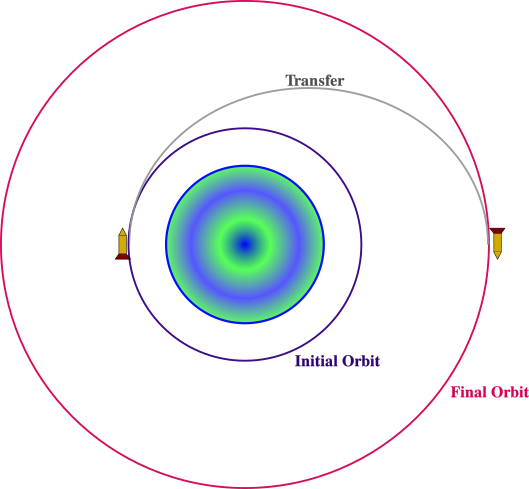
\includegraphics[scale = 0.8]{Q2_Transfer_Image.png}
	\end{figure}
	
	\pagebreak
	
	\section*{Question 3 - Trying to get back Home}
	Morty has now unfortuantely gotten separated from Rick in his travel through space. Before he got lost though, Rick gave him a GPS tracker. Although it's a little messed up because of his previous adventures, Morty is able to ping satellites and see the amount of time it takes for the signal to go from Morty to the satellite and back. 
	
	Rick however, is a little f*****. He's only given Morty 3 of the four satellite positions relative to him. They are:
	\begin{align*}
		A = \{-3141, -5926, 5358\}\\
		B = \{-9793, 2384, -6264\}\\
		C = \{3383, -2795, -288\}
	\end{align*}
	\begin{enumerate}[label = (\alph*)]
		\item Morty's first job is to figure out where the fourth satellite is. He knows Rick is enough of an a**h*** to make sure that none of the satellites are in the same octant. He also knows that the $x$, $y$ and $z$ coordinates of the satellite are probably the same. Find the position of the fourth satellite.
		\item Congratulations on finding the fourth satellite, unfortunately Morty pressed the button labelled don't press, setting off a hidden rocket inside the GPS has suddenly gone off, sending Morty tumbling through the universe. Before the GPS dies, Morty gets two sets of pings off the satellites.
		\begin{align*}
			A_1 = 28.21941442 ms \cuspac A_2 = 32.56521822 ms\\
			B_1 = 37.40539321 ms \cuspac B_2 = 37.48077648 ms\\
			C_1 = 21.88477974 ms \cuspac C_2 = 35.47581482 ms\\
			D_1 = 7.603382343 ms \cuspac D_2 = 21.38749482 ms
		\end{align*}
		\begin{enumerate}[label = (\roman*)]
			\item According to the clock, the first ping is at $t_1 = 0$ seconds, and the second is at $t_2 = 5000$ seconds (Rick is a b****). Find the direction vector and the velocity of Morty as he hurtles through space trying not to c*** his pants.
			\item Turns out, the second ping was actually sent at time $t_2 = 0.1$ seconds. Write down some of your favorite curse words to throw at Rick, and give us the direction vector and velocity of Morty.
		\end{enumerate}
		\item Morty has now landed in the orbit of Earth. His GPS splits into two pieces, a sun-sensor and a magnetic field sensor. Rick being Rick has also included a radio for Morty's use. However, for it to work, Morty needs to figure out his relative orientation to the planet. He bravely tapes the sensors to his chest pointing out, and he resigns himself to this horrible fate. Draw an approximate diagram with Morty, and show how he'd aptly describe his orienation to ground control.
	\end{enumerate}

	
	\pagebreak
	\section*{Question 4 - Bob's Cat}
	His cat has suddenly joined him. Measurements are taken every 0.5 seconds.
	\begin{enumerate}[label = (\alph*)]
		\item Given the first $n$ positions ${(x_1, y_1), (x_2, y_2), ... , (x_n, y_n)}$, estimate the true position of the cat.
		\item Obviously, noting down every position and finding the exact position every time is unfeasible (because data, duh). Give us a new expression that uses the $(n-1)_{th}$ estimation and the $n_{th}$ measurement to estimate the true position of the cat.
		\item If the measurements for the first 5 seconds are:
		\begin{equation*}
			1,2,3,4,5
		\end{equation*}
	\end{enumerate}

\backgroundsetup{contents=
\includegraphics{Anant_Logo.png}, opacity=0.1, angle=0, scale=1.5}	

\end{document}